\documentclass{beamer}
\usepackage{ucs}
\usepackage[utf8x]{inputenc}
\usepackage[T1]{fontenc}

\usepackage{graphicx}
\usepackage{tipa}

\usepackage{hyperref}
\usepackage{graphics}


\begin{document}
\title{A constraint grammar for Faroese}
\author{Trond Trosterud \\ 
University of Tromsø \begin{figure}  \scalebox{0.10}[0.10]{
\includegraphics{img/LogoEngelsk}} \end{figure} 
}

\date

\frame{\titlepage} 

\frame{\frametitle{Contents}\tableofcontents} 

\section{Introduction} 


\begin{frame}
\frametitle{Linguistic background}
\begin{itemize}
\item Lexicon and grammar
\begin{itemize}
\item Føroysk órðabók, lemmalist and inflection codes electronically accessible
\item Thráinsson, Petersen, í Lon Jacobsen, Hansen: \textit{Faroese: An overview and reference grammar} \\ \pause
\end{itemize}
\item ... but the real initiator behind this was a foggy day at Tórshavn Airport
\end{itemize}
\end{frame}

\begin{frame}
\frametitle{Background for the infrastructure}
\begin{itemize}
\item Infrastructure from the Sámi parser project (\textit{giellatekno.uit.no})
\begin{itemize}
\item The same file setup, Makefiles, etc. \\ \pause
\end{itemize}
\item Also the opposite relation:
\begin{itemize}
\item Sámi twolc testsuite taken from work on Faroese twolc
\item Experiments on Faroese dependency before Sámi dependency
\end{itemize}
\end{itemize}
\end{frame}


\begin{frame}
\frametitle{Technological background}
\begin{itemize}
\item Xerox transducer compilers for the core grammar
\begin{itemize}
\item Morphophonology: \textit{twolc} 
\item Lexicon and morphology: \textit{lexc} \\ \pause
\end{itemize}
\item Constraint grammar for sentence analysis
\begin{itemize}
\item Disambiguation, syntax and dependency: \textit{vislcg3} from Odense
\end{itemize}
\end{itemize}
\end{frame}



\frame{\frametitle{Overview of the analyser}

\begin{itemize}
\item {Lexicon}
\item Fst transducer
\item CG disambiguator
\item CG dependency
\end{itemize}
}



\section{The morphological analyser}
\begin{frame}
\frametitle{Lexicon}

\begin{itemize}
\item The analyser uses the same inflectional codes as  \textit{Føroysk orðabók} 
\begin{itemize}
\item New words annotated with the same codes may thus be added directly to the fst
\end{itemize}
\item The analyser has a dynamic compounding component (gen. sg. -> Nouns)
\end{itemize}
\end{frame}

\frame{\frametitle{Lexicon format - nouns} 
\scalebox{0.45}[0.45]{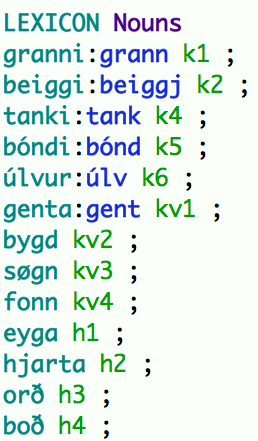
\includegraphics{img/nounlexicon.png}} \\
}

\frame{\frametitle{A name guesser for, well, names}
\begin{itemize}
\item Based upon capital first letter and non-Faroese phonotax 
\begin{itemize}
\item Initial capital
\item At least one vowel
\item The final letter cannot be a Faroese suffixal sound (\textit{a, i, u, n, m, r, s, t} (to avoid explicit case endings)
\item The putative name is then assigned Nom, Acc and Dat  \\ \pause
\end{itemize}
\item The guesser is very reliable: Of the 500 most common guesses all 500 were actually names. 
\item It is also (too) careful: Banning Faroese case suffixes from the guesser avoids analysig case-inflected forms as baseforms, but at the same time it prevents the parser from making many correct guesses. 
\end{itemize}

}

\begin{frame}
\frametitle{Morphology in three layers}
\begin{enumerate}
\item Part of speech and gender tag, morphophonological flags
\item Case and number morphology
\item Definiteness morphology
\end{enumerate}
\end{frame}


\frame{\frametitle{First layer - POS and gender} 
\scalebox{0.55}[0.55]{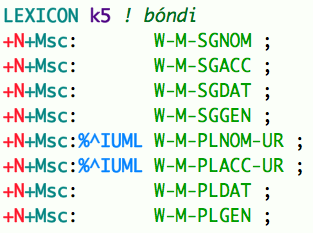
\includegraphics{img/bondi.png}} \\
}

\frame{\frametitle{Second layer - case and number} 
\scalebox{0.40}[0.40]{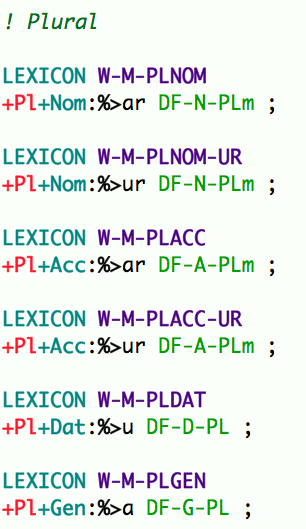
\includegraphics{img/wmplnom.png}} \\
}

\frame{\frametitle{Third layer - definiteness} 
\scalebox{0.36}[0.36]{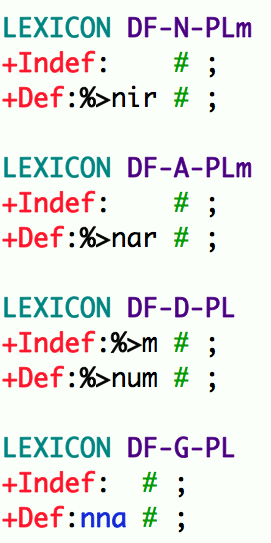
\includegraphics{img/dfnplm.png}} \\
}

\frame{\frametitle{The resulting upper and lower lexc strings} 
\scalebox{0.40}[0.40]{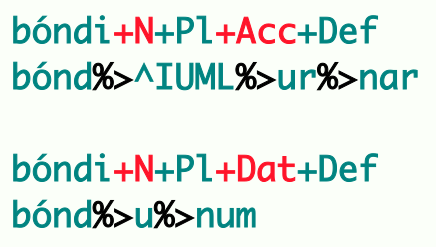
\includegraphics{img/bondi_lexc.png}} \\
}

\frame{\frametitle{The twolc i-umlaut rule} 
\scalebox{0.45}[0.45]{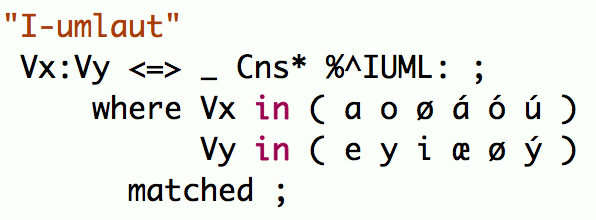
\includegraphics{img/twoliumlaut.png}} \\
}

\frame{\frametitle{The transducers} 
\scalebox{0.53}[0.53]{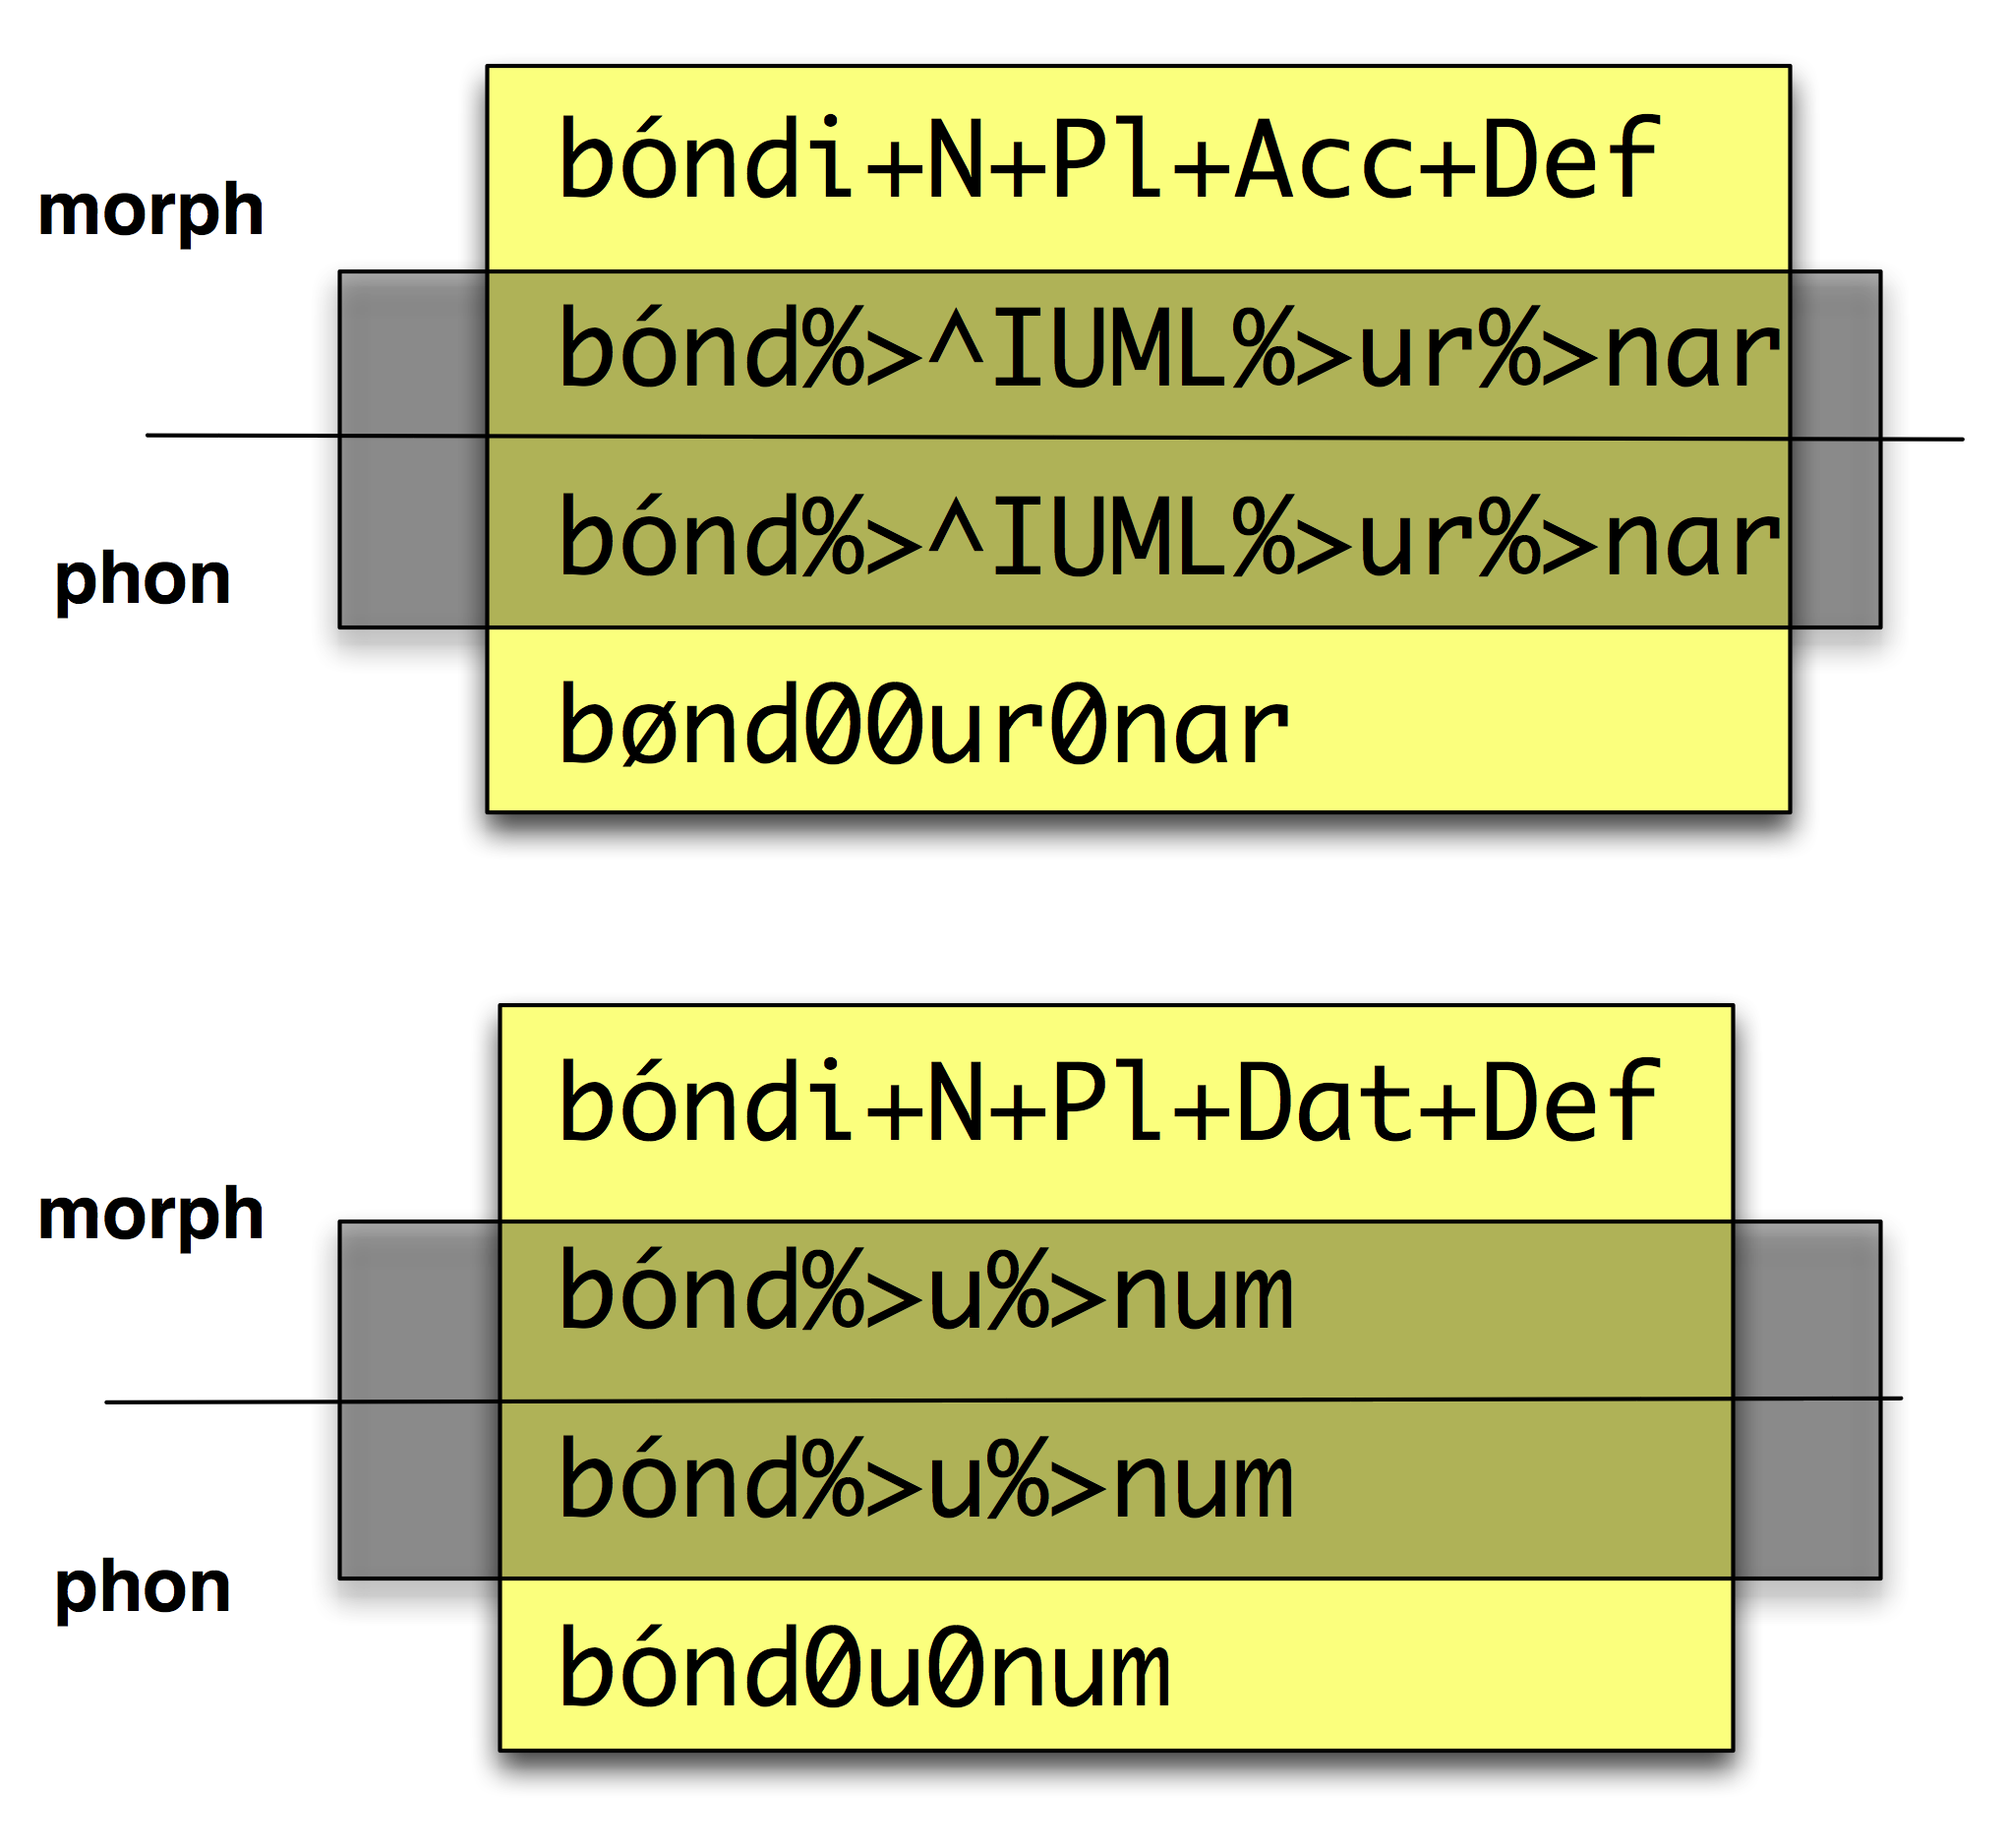
\includegraphics{img/automaton.png}} \\
}

\frame{\frametitle{The resulting paradigm for bóndi} 
\scalebox{0.33}[0.33]{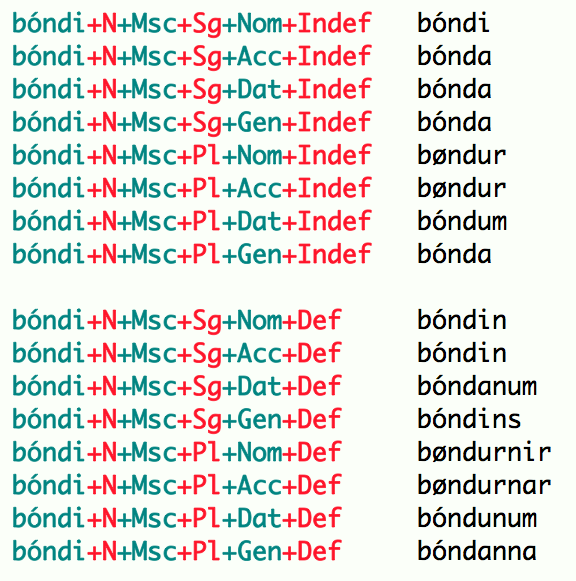
\includegraphics{img/bondiparadigm.png}} \\
}

\frame{\frametitle{Overview of twolc rules} 
\scalebox{0.29}[0.28]{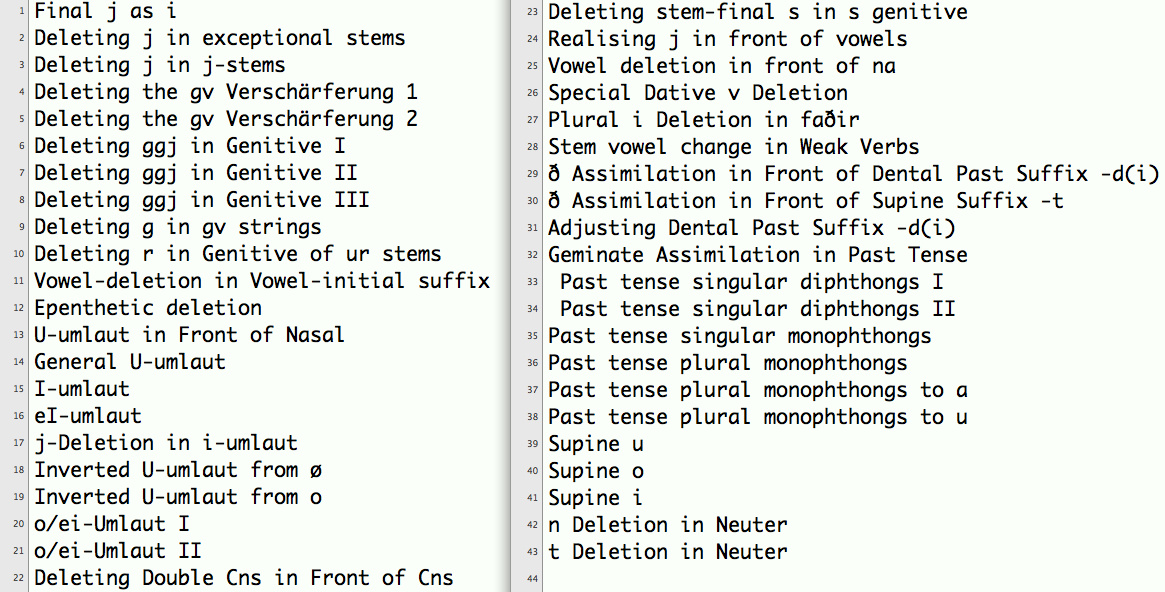
\includegraphics{img/twolrules.png}} \\
}


\begin{frame}
\frametitle{Status quo for Ffst}
\begin{itemize}
\item The parser recognises 94.3 \% of the wordforms and 63.3  \% of the wordform types in running text
\item The discrepancy indicates that Ffst handles common words better than rare ones
\item{Certain common forms are missing (some strong verbs, irregular adjective forms, comparatives (partly))}
\item{Faroese names are missing (except the most central person names), but many are taken care of by the guesser}
\end{itemize}
\end{frame}


\frame{\frametitle{The top 84 missing wordforms from an 2.7 m wd corpus} 
\scalebox{0.33}[0.33]{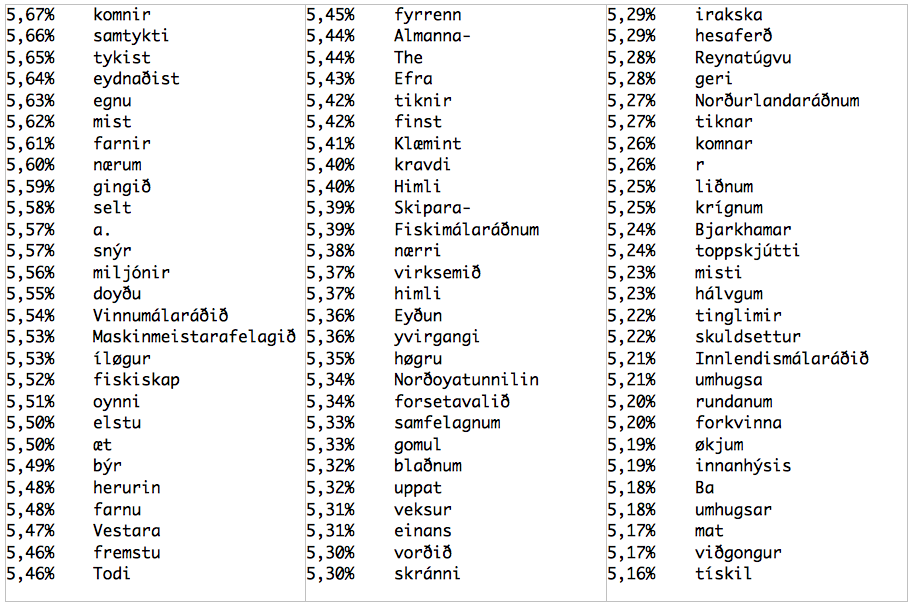
\includegraphics{img/missing.png}} \\
}


\frame{\frametitle{The missing words}
\begin{itemize}
\item The 43093 missing words represent 5.67\% of the 2.7 mill corpus. 
\item In order to reduce the number of missing words in running text by 50\%, the top 2117 wordforms of the missing list would have to be added to the analyser. \\ \pause
\item Important areas for lexicon improvement
\begin{itemize}
\item Adjectival inflection of participles, irregular adjectival forms
\item Some irregular strong verbs and verb forms
\item Faroese names (other than person names)
\item Compounded function words
\item Words missing from FÓ
\item Plain errors
\end{itemize}
\end{itemize}
}

\frame{\frametitle{The Faroese disambiguator}
The disambiguator (Fdis) consists of

\begin{itemize} 
\item 120 rules for morphological disambiguation, 
\item 49 mapping rules, 
\item 46 rules for GF-disambiguation. 
\end{itemize}
}


\frame{\frametitle{Small, but relatively efficient rule set}

\begin{table}[htdp]
%\caption{default}
\begin{center}
\begin{tabular}{|l|c|c|c|}
\hline
Parser & Rules & Input ambiguity & disambiguated output \\
\hline
North Sámi	  & 3537 & 2.42 & 1.08 \\
Norsk Bokmål  & 1964 & 2.13 & 1.17 \\
Lule Sámi	  &  832 & 2.18 & 1.21 \\
Faroese		  &  294 & 2.45 & 1.24 \\
Greenlandic	  &  518 & 2.69 & 1.42 \\
\hline
\end{tabular}
\end{center}
%\label{default}
\end{table}%
}


\begin{frame}
\frametitle{Tag unification}

The efficiency of the ruleset illustrates the efficiency of an innovation in vislcg3, namely set unification for tags. 

With the set unification operator $\$\$$ it is possible to refer to a set, so that the tag that first satisfies the set must be the same as all subsequent matches of the same set.

\begin{itemize}
\item SET NAGD = Nom Acc Gen Dat ;
\item SELECT \$\$NAGD IF (0 Det)(*1C \$\$NAGD BARRIER NOT-NP);
\end{itemize}

\end{frame}


\section{The disambiguator}

\frame{\frametitle{The disambiguator}
\begin{itemize}
\item {The bulk of the rules aims at disambiguating case, number and gender within the NP.}
\item {One clue as to determining the correct case is the choice of preposition, as it is for the human listener.}
\begin{itemize} %\\ \pause
\item Unfortunately, most Faroese prepositions subcategorise for more than one case. 
\item The choice of case is ultimately dependant upon the combination of verb (or sentence frame) and preposition. 
\item Approach: Select Acc for motion verbs and change of relationship PPs, otherwise go for Dat
\end{itemize} %\\ \pause
\item {Verb disambiguation is a key area as well}
\end{itemize}

}



\frame{\frametitle{High-frequent ambiguous words}

\begin{itemize}
\item Certain high-frequent words need special attention, 
\begin{itemize}
\item both because they get multiple interpretations in the morphological component, and 
\item for their key role in the sentence.
\end{itemize} 
\item A common strategy for such words is to write specific rules just for these words.  \\ \pause
\end{itemize} 

For Fdis, only approximately 15 such words have received special treatment until now:

\begin{description}
\item [Pronouns:] \textit{hon, vit, ..}
\item [Subjunctions:] \textit{at, ið, men, ...}
\end{description}
}


\frame{\frametitle{Verb homonymy}

\begin{itemize}
\item The Faroese verbal paradigm shows much homonymy. 
\begin{itemize}
\item Ffst specifies 3 persons in the singular (also when the conjugation in question shows homonymy), 
but there is only one plural form (no disambiguation here). 
\end{itemize} 
\end{itemize} 
}


\frame{\frametitle{Grammatical functions}

\begin{itemize}
\item Mapping of grammatical functions by
\begin{itemize}
\item morphological cues
\item word order
\end{itemize}
\item and disambiguation of grammatical functions by
\begin{itemize}
\item word order \\ \pause
\end{itemize}
\item The grammatical function tags are directional 
\begin{itemize}
\item ( @OBJ> / @<OBJ )
\end{itemize}
\item This distinction is heavily utilised in the dependency grammar.
\end{itemize}
}

\section{The dependency grammar}
\frame{\frametitle{The dependency grammar}

\begin{itemize}
\item The dependency grammar (Fdep) consists of 49 rules. 
\item The dependency grammar quite reliably delimits NPs, and the governed constituents of P and V. 
\begin{itemize}
\item Eventual errors here are due to errors in Fdis. 
\end{itemize}
\item The hard obstacles for a good depencency analyses are long-distance dependencies: 
\begin{itemize}
\item coordination and relative clauses, topicalisation.
\end{itemize}
\end{itemize}
}


\frame{\frametitle{The dependency grammar}

\begin{itemize}
\item Shortcomings in coordination and relative clause analysis, and especially the low coverage of the Ffst gives too many top nodes 
\begin{itemize}
\item 2.3 alleged clausal heads (i.e., fragments) per clause on average, compared to the correct 1 head/clause \\ \pause
\end{itemize}
\item Even with these shortcomings, the Fdep is already at this stage a good tool for research on basic dependency relations.
\end{itemize}
}

\section{Evaluation}
\frame{\frametitle{Precision and recall}

The parser was tested on a small corpus of 1033 words of unseen text from a new genre (Faroese education planning)

\begin{table}%[htdp]
%\caption{default}
%\begin{center}
\begin{tabular}{|l|r|r|r|r||r|r|r|r|r|}
\hline
Error type	& tp		& fp		& tn		& fn	& prec	 & rec.	& acc.	& F-ms. \\
\hline
Morphology  &  2048  &  369  &  2501  &  101  &  0.85  &  0.95  &  0.91  &  0.90 \\
Syntax  &  1902  &  515  &  2357  &  245  &  0.79  &  0.89  &  0.85  &  0.83 \\
Dependency  &  724  &  316  &  0  &  0  &  0.7  &  1  &  0.7  &  0.82			  \\
\hline
\end{tabular}
%\end{center}
%\label{default}
\end{table}%

\\ \pause
-> Fdis is work in progress 
}


\frame{\frametitle{Some sentences 1} 
\scalebox{0.40}[0.40]{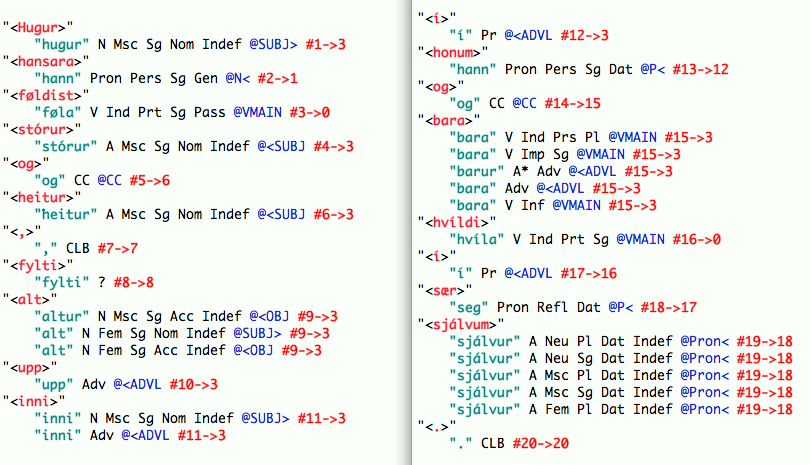
\includegraphics{img/hugur.png}} \\
}

\frame{\frametitle{Some sentences 2} 
\scalebox{0.50}[0.50]{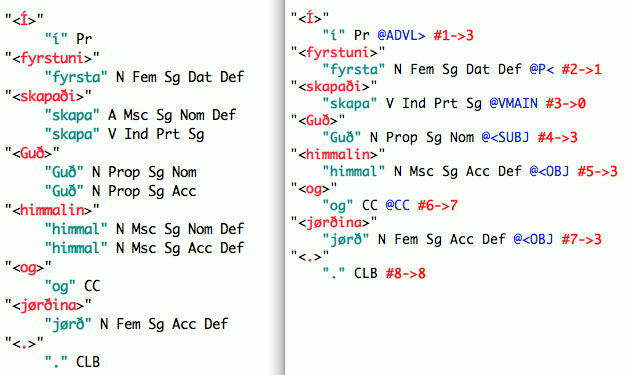
\includegraphics{img/fyrstuni.png}} \\
}

\frame{\frametitle{Some sentences 3} 
\scalebox{0.30}[0.30]{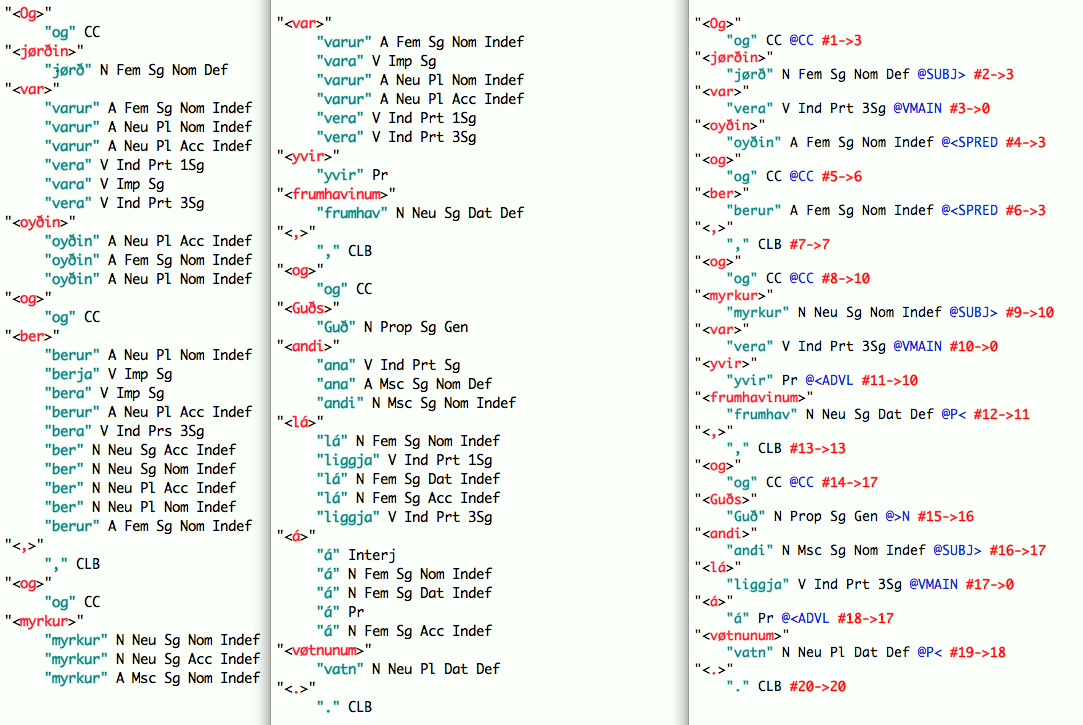
\includegraphics{img/frumhavinum.png}} \\
}


\section{Processing speed}
\frame{\frametitle{Processing speed}

\begin{itemize}
\item The bottleneck in the system is the disambiguator. 
\item Even though it is much smaller than most CG grammars, Fdis performs clearly worse than all the other parts of the pipeline.
\item The reason for this might be the extensive use of set unification.
\end{itemize}

\begin{table}[htdp]
\caption{Processing speed, measured on 100000 words of running text, on a 2,4 GHz laptop}
\begin{center}
\begin{tabular}{|l|l|r|}
\hline
Process & Program & Words/sec \\
\hline
Preprocessing & perl &10446 \\
Morphological lookup & fst & 42992 \\
Postprocessing & perl & 13017 \\
Disambiguation & vislcg3 & 2042 \\
Dependency & vislcg3 & 18814 \\
\hline
\end{tabular}
\end{center}
\label{time}
\end{table}%




}


\frame{\frametitle{Conclusion}

\begin{itemize}
\item The Faroese grammatical analyser presented here is still in the making. \\ \pause
\item It still shows that with a modest number of CG rules, one may achive results good enough for several languaguage processing tasks.  \\ \pause
\item Future improvements of the analyser will concentrate upon key parts of the Ffst, upon disambiguation of complex syntactic patterns, and upon the dependency analysis of coordination and relative clauses. \\ \pause
\item The parser is eagerly waiting for cooperation partners, and interesting work tasks
\end{itemize}
}

\frame{\frametitle{}
\begin{center}
Thank you!
\end{center}
}	
\end{document}
